\documentclass{article}

\usepackage{url,graphicx,tabularx,array,geometry, hyperref}
\usepackage{listings}
\lstset{basicstyle=\ttfamily,
  showstringspaces=false,
  breaklines=true
}
\usepackage{fullpage}
\usepackage{fancyvrb}
\usepackage{framed}
\usepackage{lastpage}
\usepackage{fancyhdr}
\usepackage{float}


\renewcommand{\headrulewidth}{0pt}
\setcounter{secnumdepth}{0}

\setlength{\parskip}{1ex} %--skip lines between paragraphs
\setlength{\parindent}{0pt} %--don't indent paragraphs
\setlength{\headheight}{15.2pt}

\pagestyle{fancy}

\renewcommand{\headrulewidth}{0pt}
\lhead{  }
\lfoot{Lab 1: TCP Congestion Control}
\rfoot{page \thepage\ of \pageref{LastPage}}

\renewcommand{\familydefault}{\sfdefault}
\begin{document}



\begin{titlepage}
\begin{center}
\textsc{\huge \bfseries Advanced Networking 2018}\\[1.5cm]
\textsc{\large Lab \#1: TCP Congestion Control}\\[1.5cm]
\textsc{\huge Report}\\[1.5cm]
\textsc{\huge \bfseries GROUP: 12}\\[1.5cm]
\textsc{\large{\textbf{Authors:}\\ Adrien Raulot, adrien.raulot@os3.nl\\ Kotaiba Alachkar, kotaiba.alachkar@os3.nl}}

\textsc{\large University of Amsterdam}
\end{center}
\end{titlepage}

\subsection{Q1.1 Plot a graph showing CWND versus time from 0.0s to
100.0s.}

\begin{figure}[H]
\centering
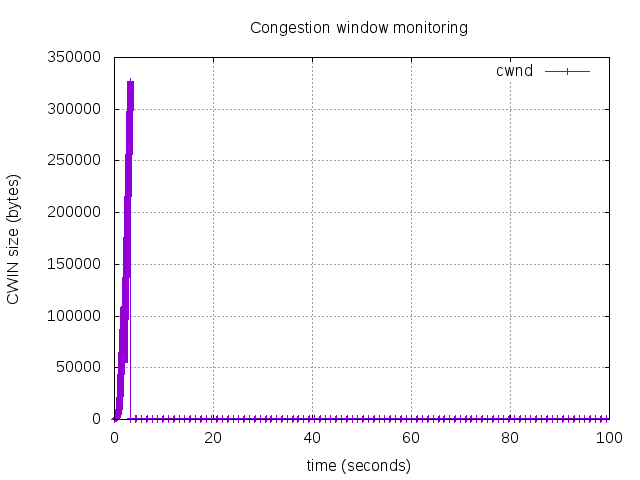
\includegraphics[width=12cm]{figures/cwndReno.png}
\caption{Reno CWND time 0.0s to 100.0s}
\end{figure}



\begin{figure}[H]
\centering
 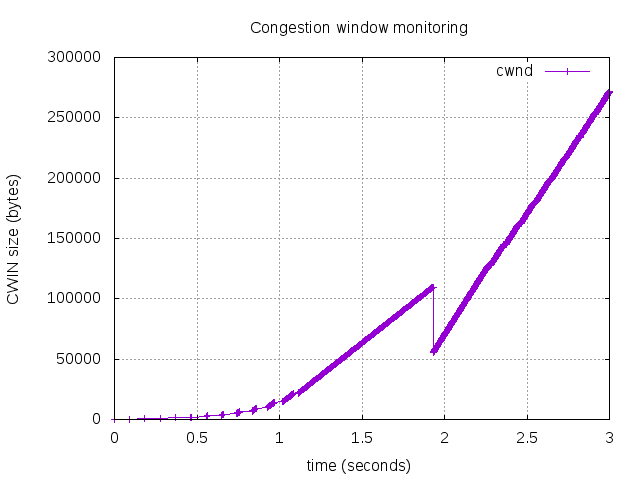
\includegraphics[width=12cm]{figures/cwndReno_1.png}
\caption{Reno CWND time 0.0s to 3.0s}
\end{figure}



\begin{figure}[H]
\centering
 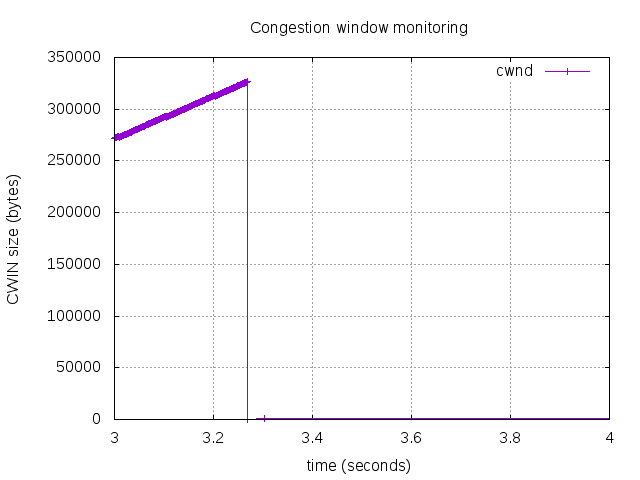
\includegraphics[width=12cm]{figures/cwndReno_2.png}
\caption{Reno CWND time 3.0s to 4.0s}
\end{figure}



\begin{figure}[H]
\centering
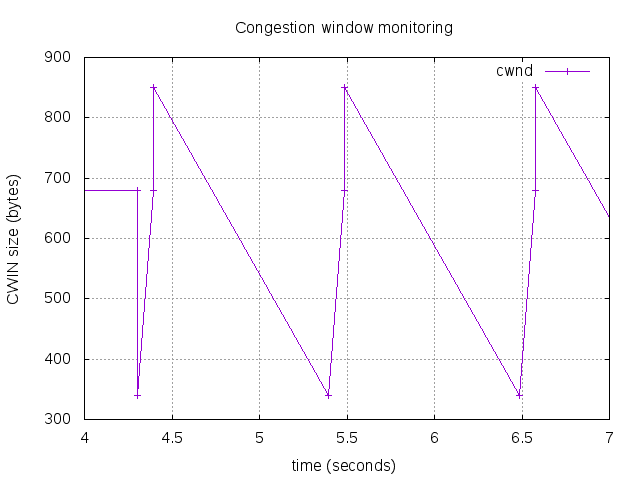
\includegraphics[width=12cm]{figures/cwndReno_3.png}
\caption{Reno CWND time 4.0s to 7.0s}
\end{figure}






\subsection{Q1.2 Plot a graph showing SSTH versus time from 0.0s to
100.0s.}


\begin{figure}[H]
\centering
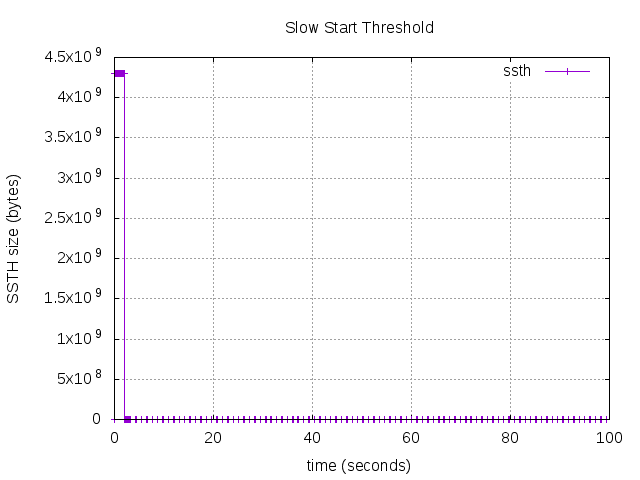
\includegraphics[width=12cm]{figures/ssthReno.png}
\caption{Reno SSTH time 0.0s to 100.0s}
\end{figure}




\subsection{Q1.3 Find the points where the slow-start,
congestion-avoidance, fast retransmit/fast recovery states begin.}

\begin{table}[H]
\centering
\begin{tabular}{|c|p{25mm}|p{20mm}|c|c|}
\hline Time (s)    & Current CWND (bytes)    & New CWND (bytes)    & New State    & Event \\
\hline 0.0905768   & 0                       & 340          & slow-start          & connection initialization\\
\hline 1.93189     & 109480                  & 55590        & fast-recovery       & duplicate ACK\\
\hline 3.26916     & 326570                  & 340          & slow-start          & timeout\\ 
\hline 4.39503     & 680                     & 850          & congestion avoidance   & $cwnd \geq ssht$ \\
\hline  
\end{tabular} 
\end{table}


\subsection{Q1.4 Plot a graph showing CWND versus time from 0.0s to
100.0s.}


\begin{figure}[H]
\centering
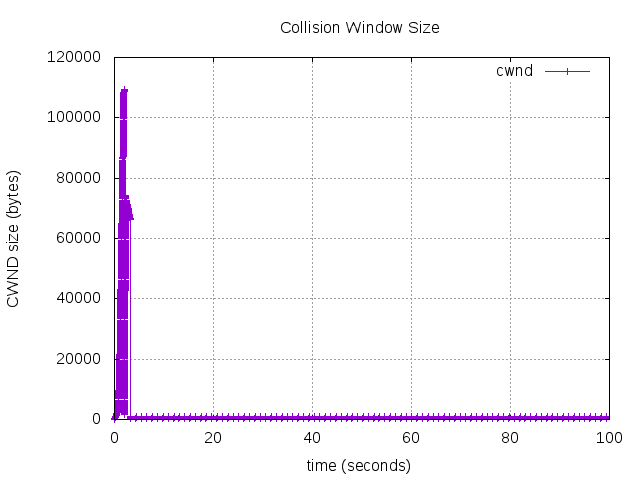
\includegraphics[width=12cm]{figures/cwndWestwood.png}
\caption{Westwood CWND time 0.0s to 100.0s}
\end{figure}



\begin{figure}[H]
\centering
 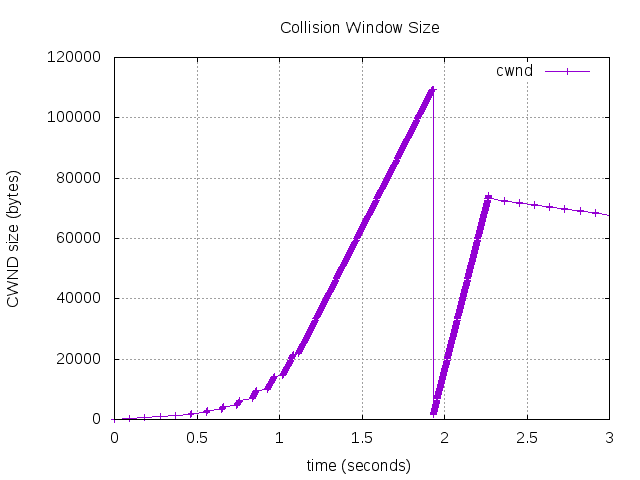
\includegraphics[width=12cm]{figures/cwndWestwood_1.png}
\caption{Westwood CWND time 0.0s to 3.0s}
\end{figure}



\begin{figure}[H]
\centering
 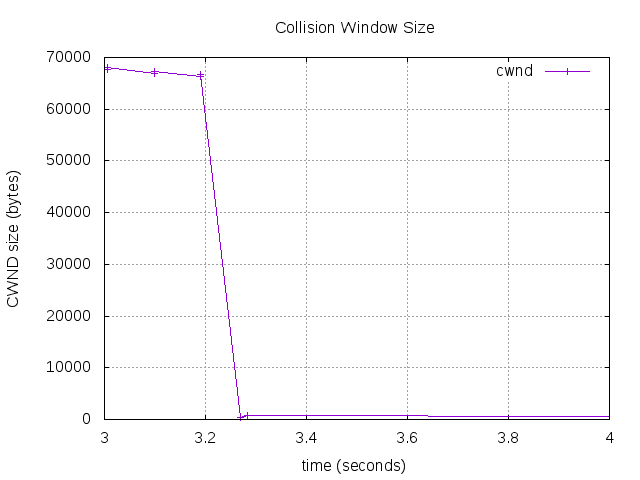
\includegraphics[width=12cm]{figures/cwndWestwood_2.png}
\caption{Westwood CWND time 3.0s to 4.0s}
\end{figure}



\begin{figure}[H]
\centering
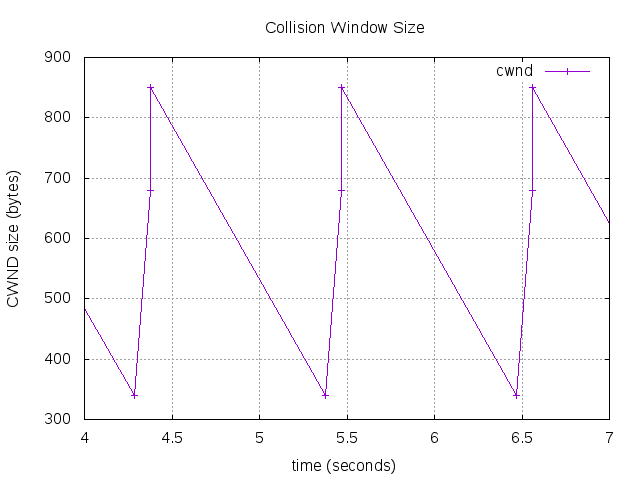
\includegraphics[width=12cm]{figures/cwndWestwood_3.png}
\caption{Westwood CWND time 4.0s to 7.0s}
\end{figure}




\subsection{Q1.5 Plot a graph showing SSTH versus time from 0.0s to
100.0s.}


\begin{figure}[H]
\centering
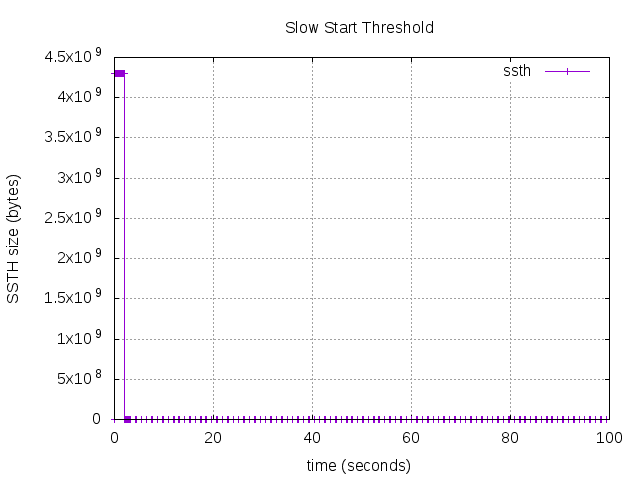
\includegraphics[width=12cm]{figures/ssthWestwood.png}
\caption{Westwood SSTH time 0.0s to 100.0s}
\end{figure}

\subsection{Q1.6 Find the points where the slow-start,
congestion-avoidance, fast retransmit/fast recovery states begin.}

\begin{table}[H]
\centering
\begin{tabular}{|c|p{25mm}|p{20mm}|c|c|}
\hline Time (s)    & Current CWND (bytes)    & New CWND (bytes)    & New State    & Event \\
\hline 0.0905768   & 0                       & 340          & slow-start          & connection initialization\\
\hline 1.93189     & 109480                  & 1700        & congestion avoidance   & duplicate ACK\\
\hline 3.19086     & 66640                  & 340          & slow-start          & timeout\\ 
\hline 4.3752     & 680                     & 850          & congestion avoidance   & $cwnd \geq ssht$ \\
\hline  
\end{tabular} 
\end{table}



\subsection{Q1.7 Discuss and motivate the differences you observe
between the NewReno and this algorithm.} %to-do: fix this in proper way

NewReno : Limits unknown packets being received. Limits the congestion window, and reset itself to a slow-start state. but if 3 of the same packets are received, it will halve the window, instead of reducing it to one. It changes the slow start threshold equal to that of the congestion window.
\\
\textbf{The algorithm that we used}
Westwood: A newer version of Reno, and another commonly used one. It controls parameters better, helping out streaming and overall quality of browsing the internet. One of the most 'fair' algorithms out there, and is one of the most efficient algorithms to date. 

The state machines also seem to differ because New Reno stays in Slow start. However, Westwood has an extra set of slow start and congestion avoidance after the first drop. 


\subsection{Q2.1 Plot a graph showing the CWND and ssthresh versus time
with all the data you get. These two metrics are in one graph.}

\begin{figure}[H]
\centering
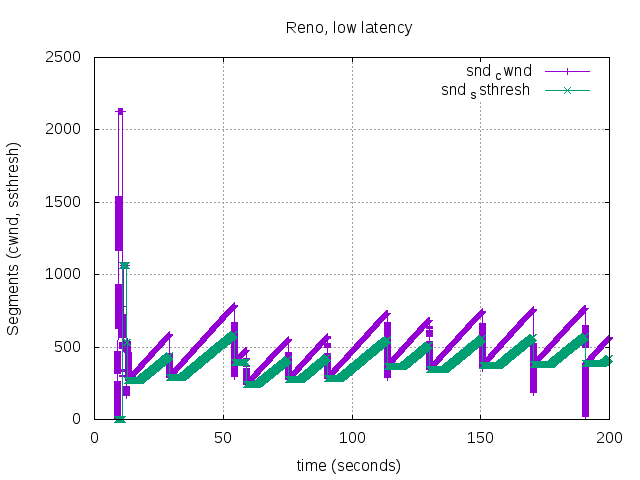
\includegraphics[width=12cm]{figures/RenoLLcwnd.png}
\caption{Reno Low Latency CWND and ssthresh versus time}
\end{figure}

\subsection{Q2.2 Briefly discuss the changing process.}

The starting point for CWND and SSTRESH are in default value. However, after the slow start phase the protocol enters in the congestion avoidance which makes the window to slowly increase until it gets multiple duplicate ACKs which triggers the fast recovery phase.  During this transition the SSTRESH is cut in half and the congestion window is set to the new SSTRESH plus 3 MSS. The protocol transitions back to congestion avoidance and the congestion window slowly increases until it receives multiple duplicate ACKs after a new ACK is received. This will keep happening and repeating until the end of the experiment.


\subsection{Q2.3 Plot a graph showing CWND versus time with all the data
you get.}

\begin{figure}[H]
\centering
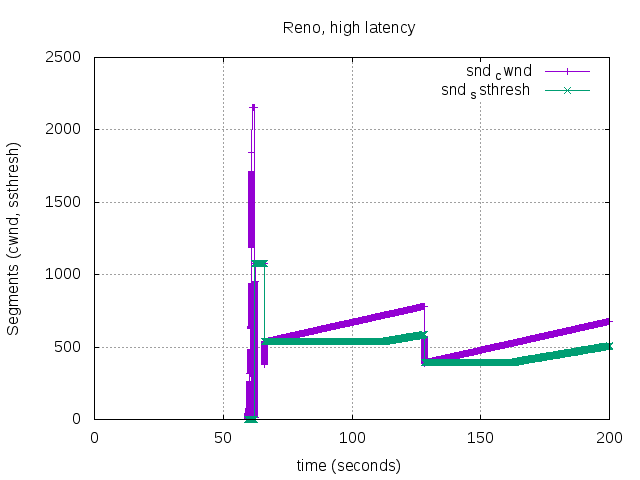
\includegraphics[width=12cm]{figures/RenoHLcwnd.png}
\caption{Reno High Latency CWND and ssthresh versus time}
\end{figure}

\subsection{Q2.4 Compare this graph with the one from Q2.1, show the difference between these two
graphs.}

These two graphs both display the same pattern, although in Q2.3 the pattern much longer than in Q1.1. That happened because of the high latency. It takes longer for the source to be informed of packet loss at the sink.

\subsection{Q2.5 Plot a graph showing CWND and ssthresh versus time with
all the data you get.}

\begin{figure}[H]
\centering
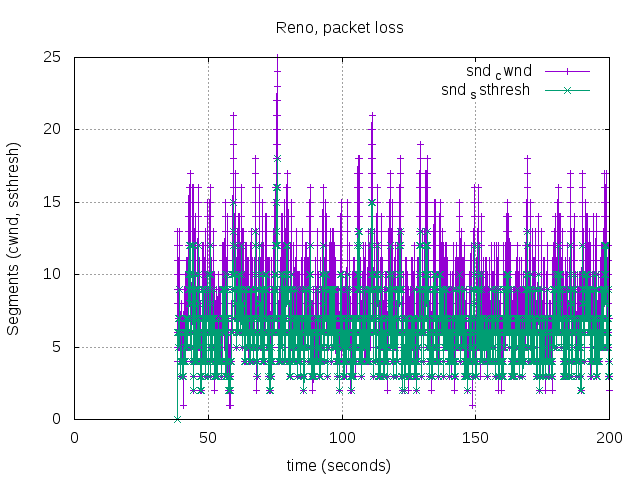
\includegraphics[width=12cm]{figures/RenoPLcwnd.png}
\caption{Reno Packet Loss CWND and ssthresh versus time}
\end{figure}

\subsection{Q2.6 Compare this graph with the graph of Q2.1 discuss and point out the major differences.}

Due to the 3\% packet loss, duplicate ACKs are observed. Reno interprets it as congestion and adapts the CWND and SSTRESH accordingly and more frequently, resulting in a high pattern variations in the graph.

\subsection{Q2.7 Zoom in the graph of this scenario (plot some parts of this scenario in a short duration, 10 or 20 seconds). Briefly explain the changing process.}

\begin{figure}[H]
\centering
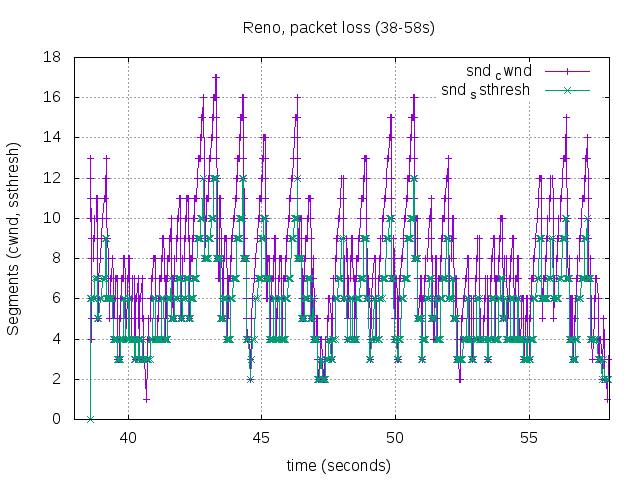
\includegraphics[width=12cm]{figures/RenoPLcwndZoom.png}
\caption{Reno Packet Loss CWND and ssthresh versus time (zoomed in)}
\end{figure}

In this graph (zoomed 38-58 seconds) we can notice that The SSTRESH can be seen to be constantly readjusted, and due to the 3\% packet loss, TCP protocol appears to constantly shifting between phases.






\subsection{Q2.8 Show a screen capture of the real throughput in this
scenario.}

\begin{figure}[H]
\centering
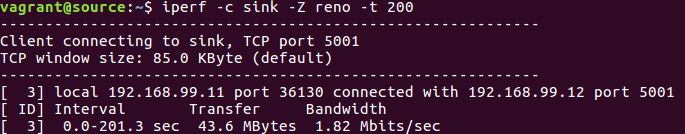
\includegraphics[width=12cm]{figures/renoScreenCapture.png}
\caption{Reno Packet Loss CWND and ssthresh screen capture}
\end{figure}

\subsection{Q2.9 Plot a graph showing CWND and ssthresh versus time with
all the data you get.}

\begin{figure}[H]
\centering
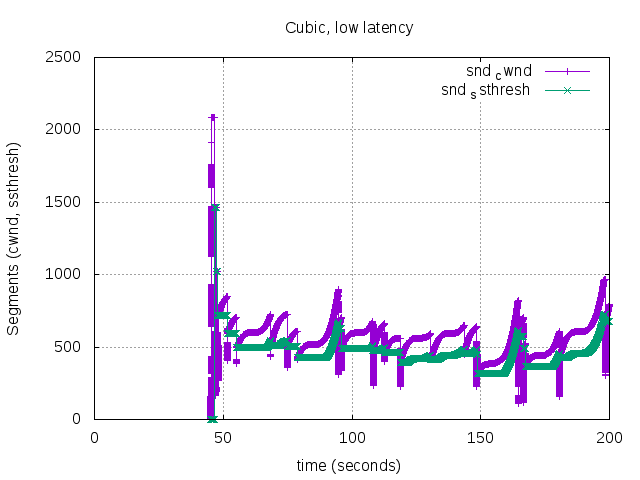
\includegraphics[width=12cm]{figures/CubicLLcwnd.png}
\caption{Cubic Low Latency CWND and ssthresh versus time}
\end{figure}

\subsection{Q2.10 Compare this graph with the graph of Q2.1 discuss and point out the major differences.}

The congestion window of Reno is calculated differently from Cubic, the latter sets the multiplicative window decrease to 0.7, while Reno takes half. The result is the CWND grows in a cubic function fashion and that can be observed on this graph.

\subsection{Q2.11 Plot a graph showing CWND and ssthresh versus time
with all the data you get.}

\begin{figure}[H]
\centering
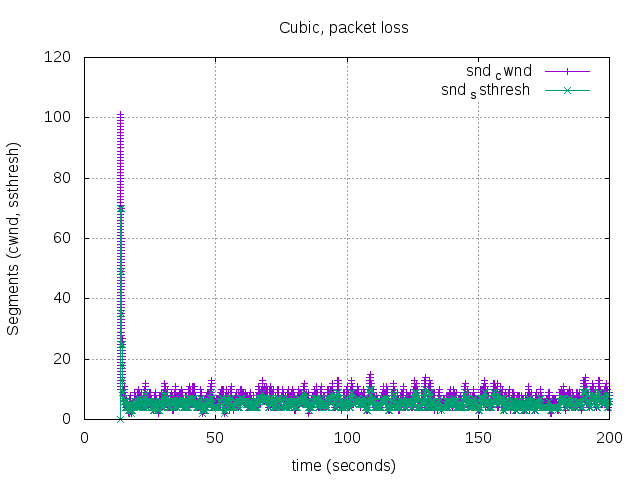
\includegraphics[width=12cm]{figures/CubicPLcwnd.png}
\caption{Cubic Packet Loss CWND and ssthresh versus time}
\end{figure}

\subsection{Q2.12 Compare this graph with the graph of scenario three
and show the differences.}

We can clearly noticed that in scenario 3, the graph appears very crowded. However, The peaks points of the graphs are not high as in scenario 3, a possible explanation for that is that the overall throughput is lower.


\subsection{Q2.13 Zoom in the graph of this scenario (plot some parts of
this scenario in a short duration, 10 or 20 seconds). Briefly explain
the changing process and compare it with the graph of Q2.7.}

\begin{figure}[H]
\centering
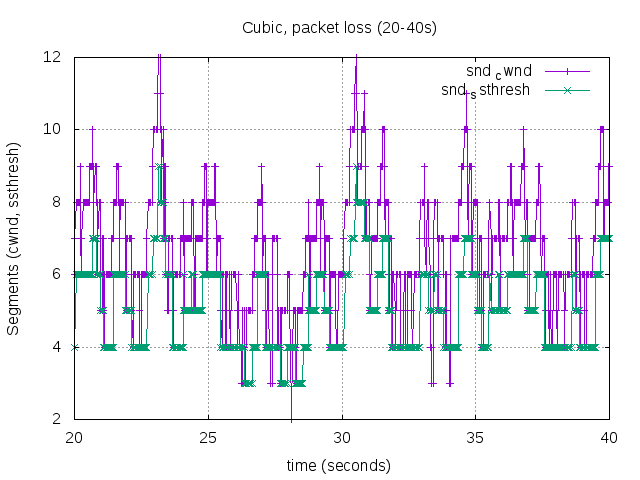
\includegraphics[width=12cm]{figures/CubicPLcwndZoom.png}
\caption{Cubic Packet Loss CWND and ssthresh versus time (zoomed in)}
\end{figure}

We derive from that Reno update its congestion window and slow start threshold more often. However, Cubic in the same time frame has fewer changes in the congestion window. 

\subsection{Q2.14 Show a screen capture of the real throughput and
compare it with throughput of Q2.8. Tell the differences.}

\begin{figure}[H]
\centering
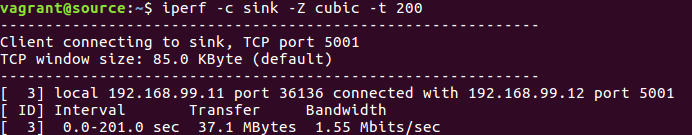
\includegraphics[width=12cm]{figures/cubicScreenCapture.png}
\caption{Cubic Packet Loss CWND and ssthresh screen capture}
\end{figure}

We can clearly notice by comparing these two screen shots that the throughput in case of Reno is higher than Cubic. 

\subsection{Q3.1 Explain what an LFN network is. Change the simulation parameters to your likings and demonstrate that TcpNewReno is not suitable for LFN networks.}

First off, Bandwidth-delay product (BDP) is the product of a data link’s capacity (in bps) and its round-trip delay time (in seconds). The result is the maximum amount of data (bits or bytes) on the network at any given time, that is data that has been transmitted but not yet acknowledged. Described in RFC 1072, networks with a BDP larger than 12500 bytes are considered as Long Fat Networks (LFN).

\subsection{Q3.2 Explain SACK does. Change the simulation parameters to
your likings and demonstrate the performance improvement with SACK.}

Described in RFC 2018, SACK stands for Selective Acknowledgement, a mechanism that can help overcome the problem of a data sender only being to learn about a single lost packet per round trip time. The SACK option is included in a TCP segment sent from the data receiver to the data sender and informs the latter of non-contiguous blocks of data that have been received and queued.

\begin{lstlisting}[language=bash]
./waf --run tcp-variants-comparison --command-template="%s --tracing=1 
--pcap_tracing=1 --sack=1 --duration=100"
\end{lstlisting}

\begin{figure}[H]
\centering
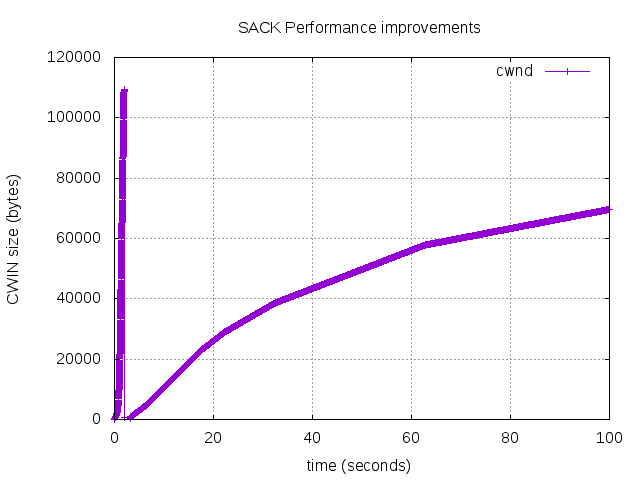
\includegraphics[width=12cm]{figures/SackTCPVariantsComparison.png}
\caption{Selective Acknowledgment Performance improvement}
\end{figure}




\subsection{Q3.3 Explain with TCP fairness is. Show the effect of
multiple flows in the simulation.}


TCP fairness is congestion control mechanisms for new network transmission protocols or peer-to-peer applications that must interact well with TCP. It requires that a new protocol receives no larger share of the network than a comparable TCP flow. This is important as TCP is the dominant transport protocol on the Internet, and if new protocols acquire unfair capacity they tend to cause problems such as congestion collapse. (Source: Wikipedia) 




\subsection{Q3.4 Replicate scenario 3 of the emulation: packet loss of
3\%, delay of 50 ms and transfer duration of 200sec. Use TcpNewReno.
Compare the two results.}

\begin{figure}[H]
\centering
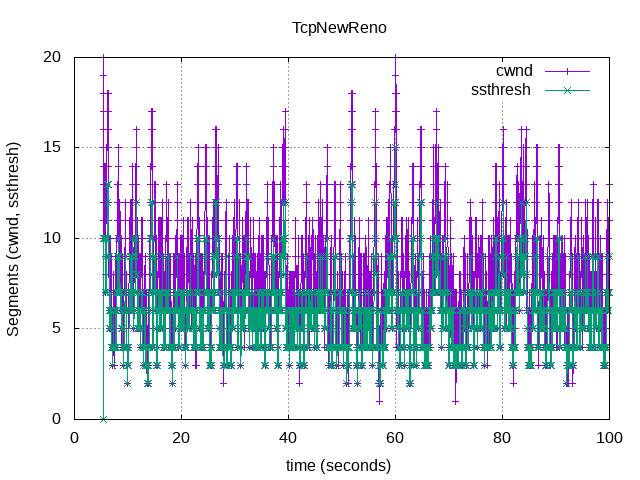
\includegraphics[width=12cm]{figures/tcpnewreno.png}
\caption{TCP New Reno with Packet Loss}
\end{figure}


As we see above the results are differences compared to scenario 3. This figure demonstrate the size of cwnd and sshthresh. However, scenario 3 shows the amount of segments which are sent. It turns to be more than the size of cwnd in bytes. 






\subsection{Q3.5 After these experiments, please briefly describe the
difference between simulation and emulation?}

An emulation emulates real working machines and runs the full software stack of the protocol in a real working environment and it runs in real time and takes into account all conditions, even those unintended. However, the simulation is a mathematical model intended to simulate conditions and apply the rules of the protocol to those conditions. It is more isolated and is more of a logical run of the protocol and it does not function as a real working environment and does not necessarily run in real time and .

\end{document}
% Template for table used in Task 1
%
% \begin{table}
% \begin{tabular}{|c|p{25mm}|p{20mm}|c|c|}
% \hline Time (s)    & Current CWND (bytes)    & New CWND (bytes)    & New State    & Event \\
% \hline ...         &              &          &             & \\ 
% \hline ...         &              &          &             & \\ 
% \hline ...         &              &          &             & \\ 
% \hline ...         &              &          &             & \\   
% \hline  
% \end{tabular} 
% \end{table}